\chapter{SATCOM for UAV Communication}
\section{SATCOM Introduction}
Satellite Communication (SATCOM) can be utilized in applications where the user wants the data from the UAV to be accessed immediately without wanting the UAV to return. It would benefit greatly in surveillance applications in remote locations, where cellular resources are unvailable.

3GPP community is also trying to incorporate SATCOM with cellular technologies, especially 5G, given its low latency and high datarate capabilities. In a typical 5G cellular network, we have a UE (user equipment) communicating with the 5G core network via the gNB (i.e base station) to access the data and voice services as shown in the Figure \ref{Conventional_5G}.

\begin{figure}[h!]
\centering
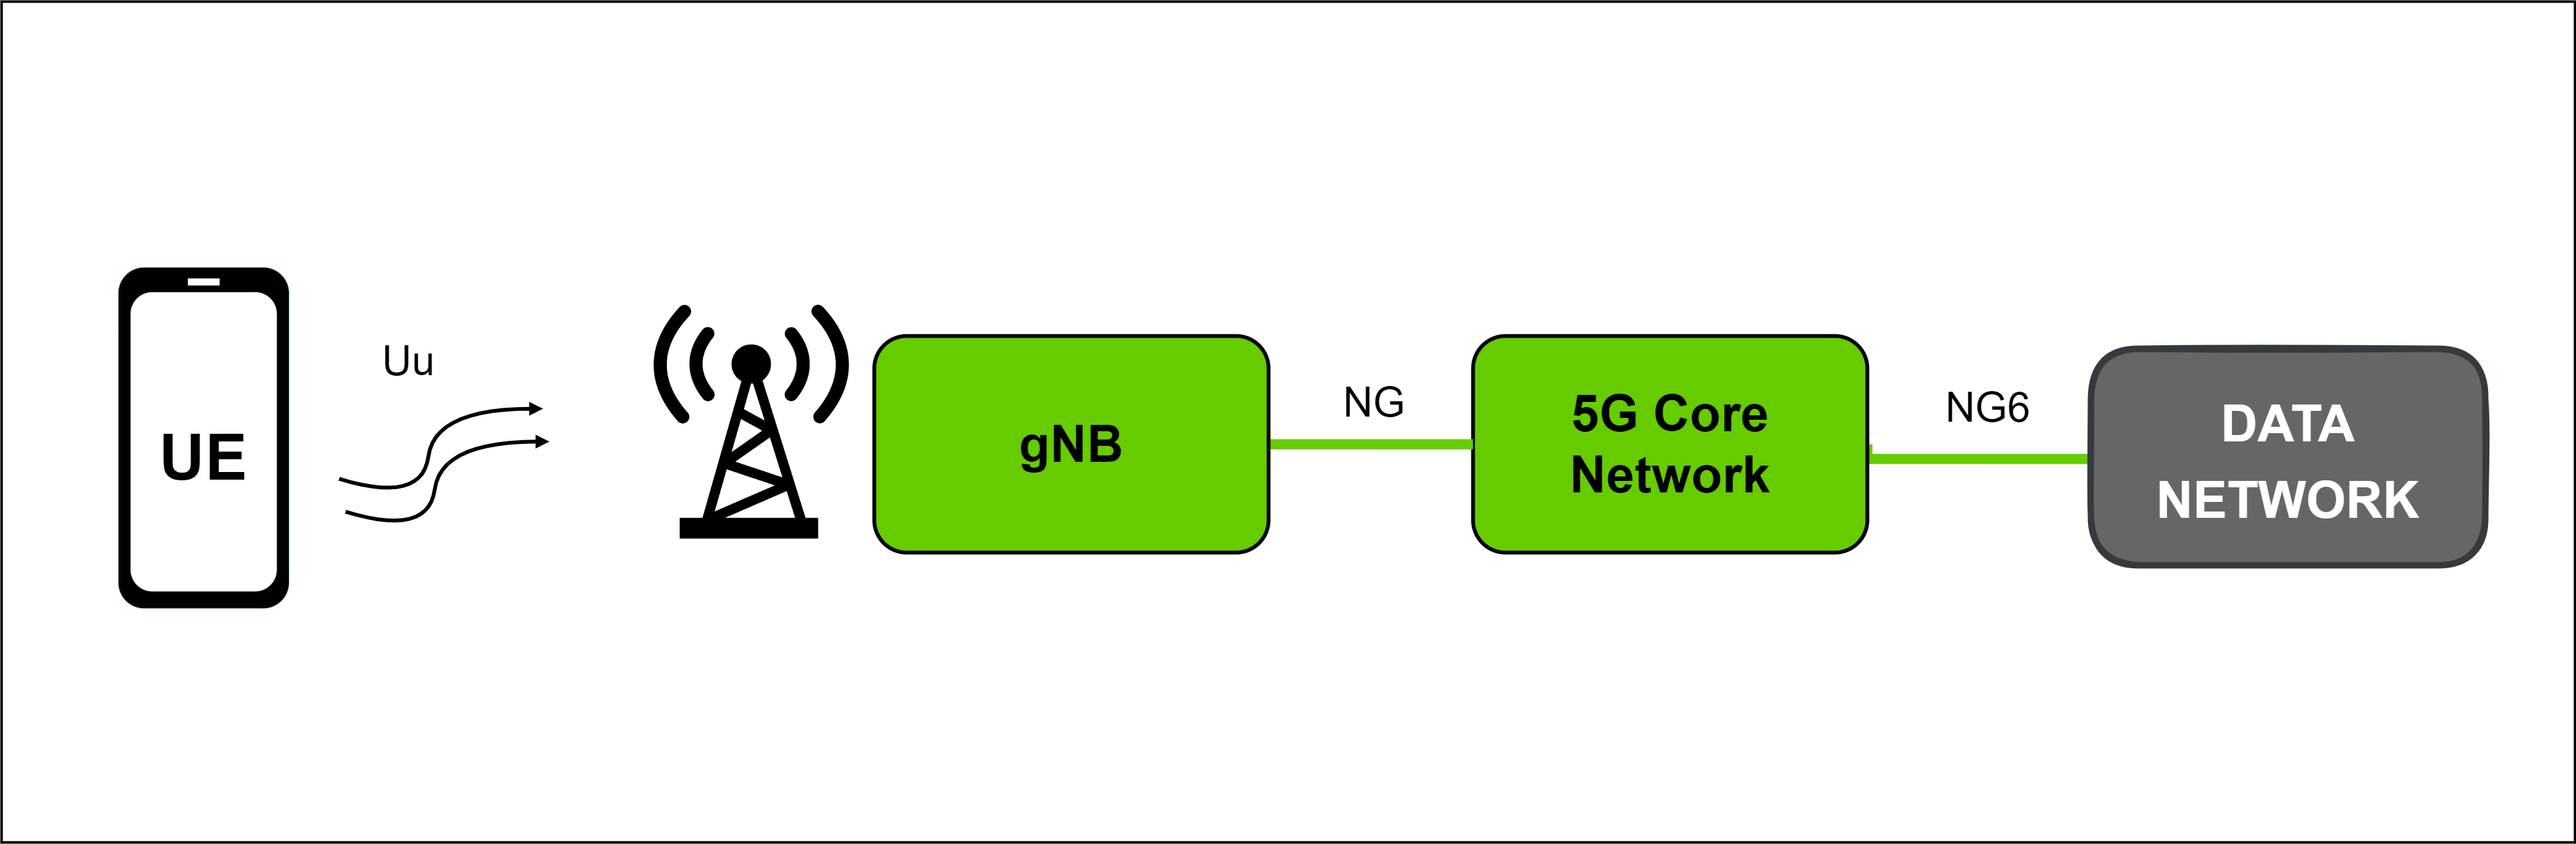
\includegraphics[width=12cm]{./Figures/Conventional_5G.png}
\caption{Conventional 5G-NR system}
\label{Conventional_5G}
\end{figure}

However, in case where our user equipment is an UAV, it may not be always reachable from its nearest gNB (for example in remote areas like forests, mountainous terrain, etc). This is where SATCOM would provide a non-terrestial network infrastructure, enabling communication with such remote devices. Furthermore, latest advancements in the satellite communications have overcome previous constraints. New generation of Low Earth Orbit (LEO) constellations have lessened satellite communications latency, and technological improvements in Geostationary (GEO) satellites have provided high throughput and increased the reliability of GEO satellites.

A SATCOM infrastucture consist of one or more satellites. Satellites are Spaceborne vehicles orbiting the earth in Low Earth Orbits (LEO), Medium Earth Orbits (MEO), or Geostationary Earth Orbit (GEO). A non-terrestrial network refers to a network, or segment of networks using RF resources on board a satellite.

A Transparent satellite based NG-RAN architecture is as shown in Figure \ref{SATCOM_figure}. Here, the Uu Air interface between the user equipment (i.e. UAV) and the gNB is replaced by a satellite link. This ensures connectivity everywhere on the surface which is under coverage of the satellite.

\begin{figure}[h!]
\centering
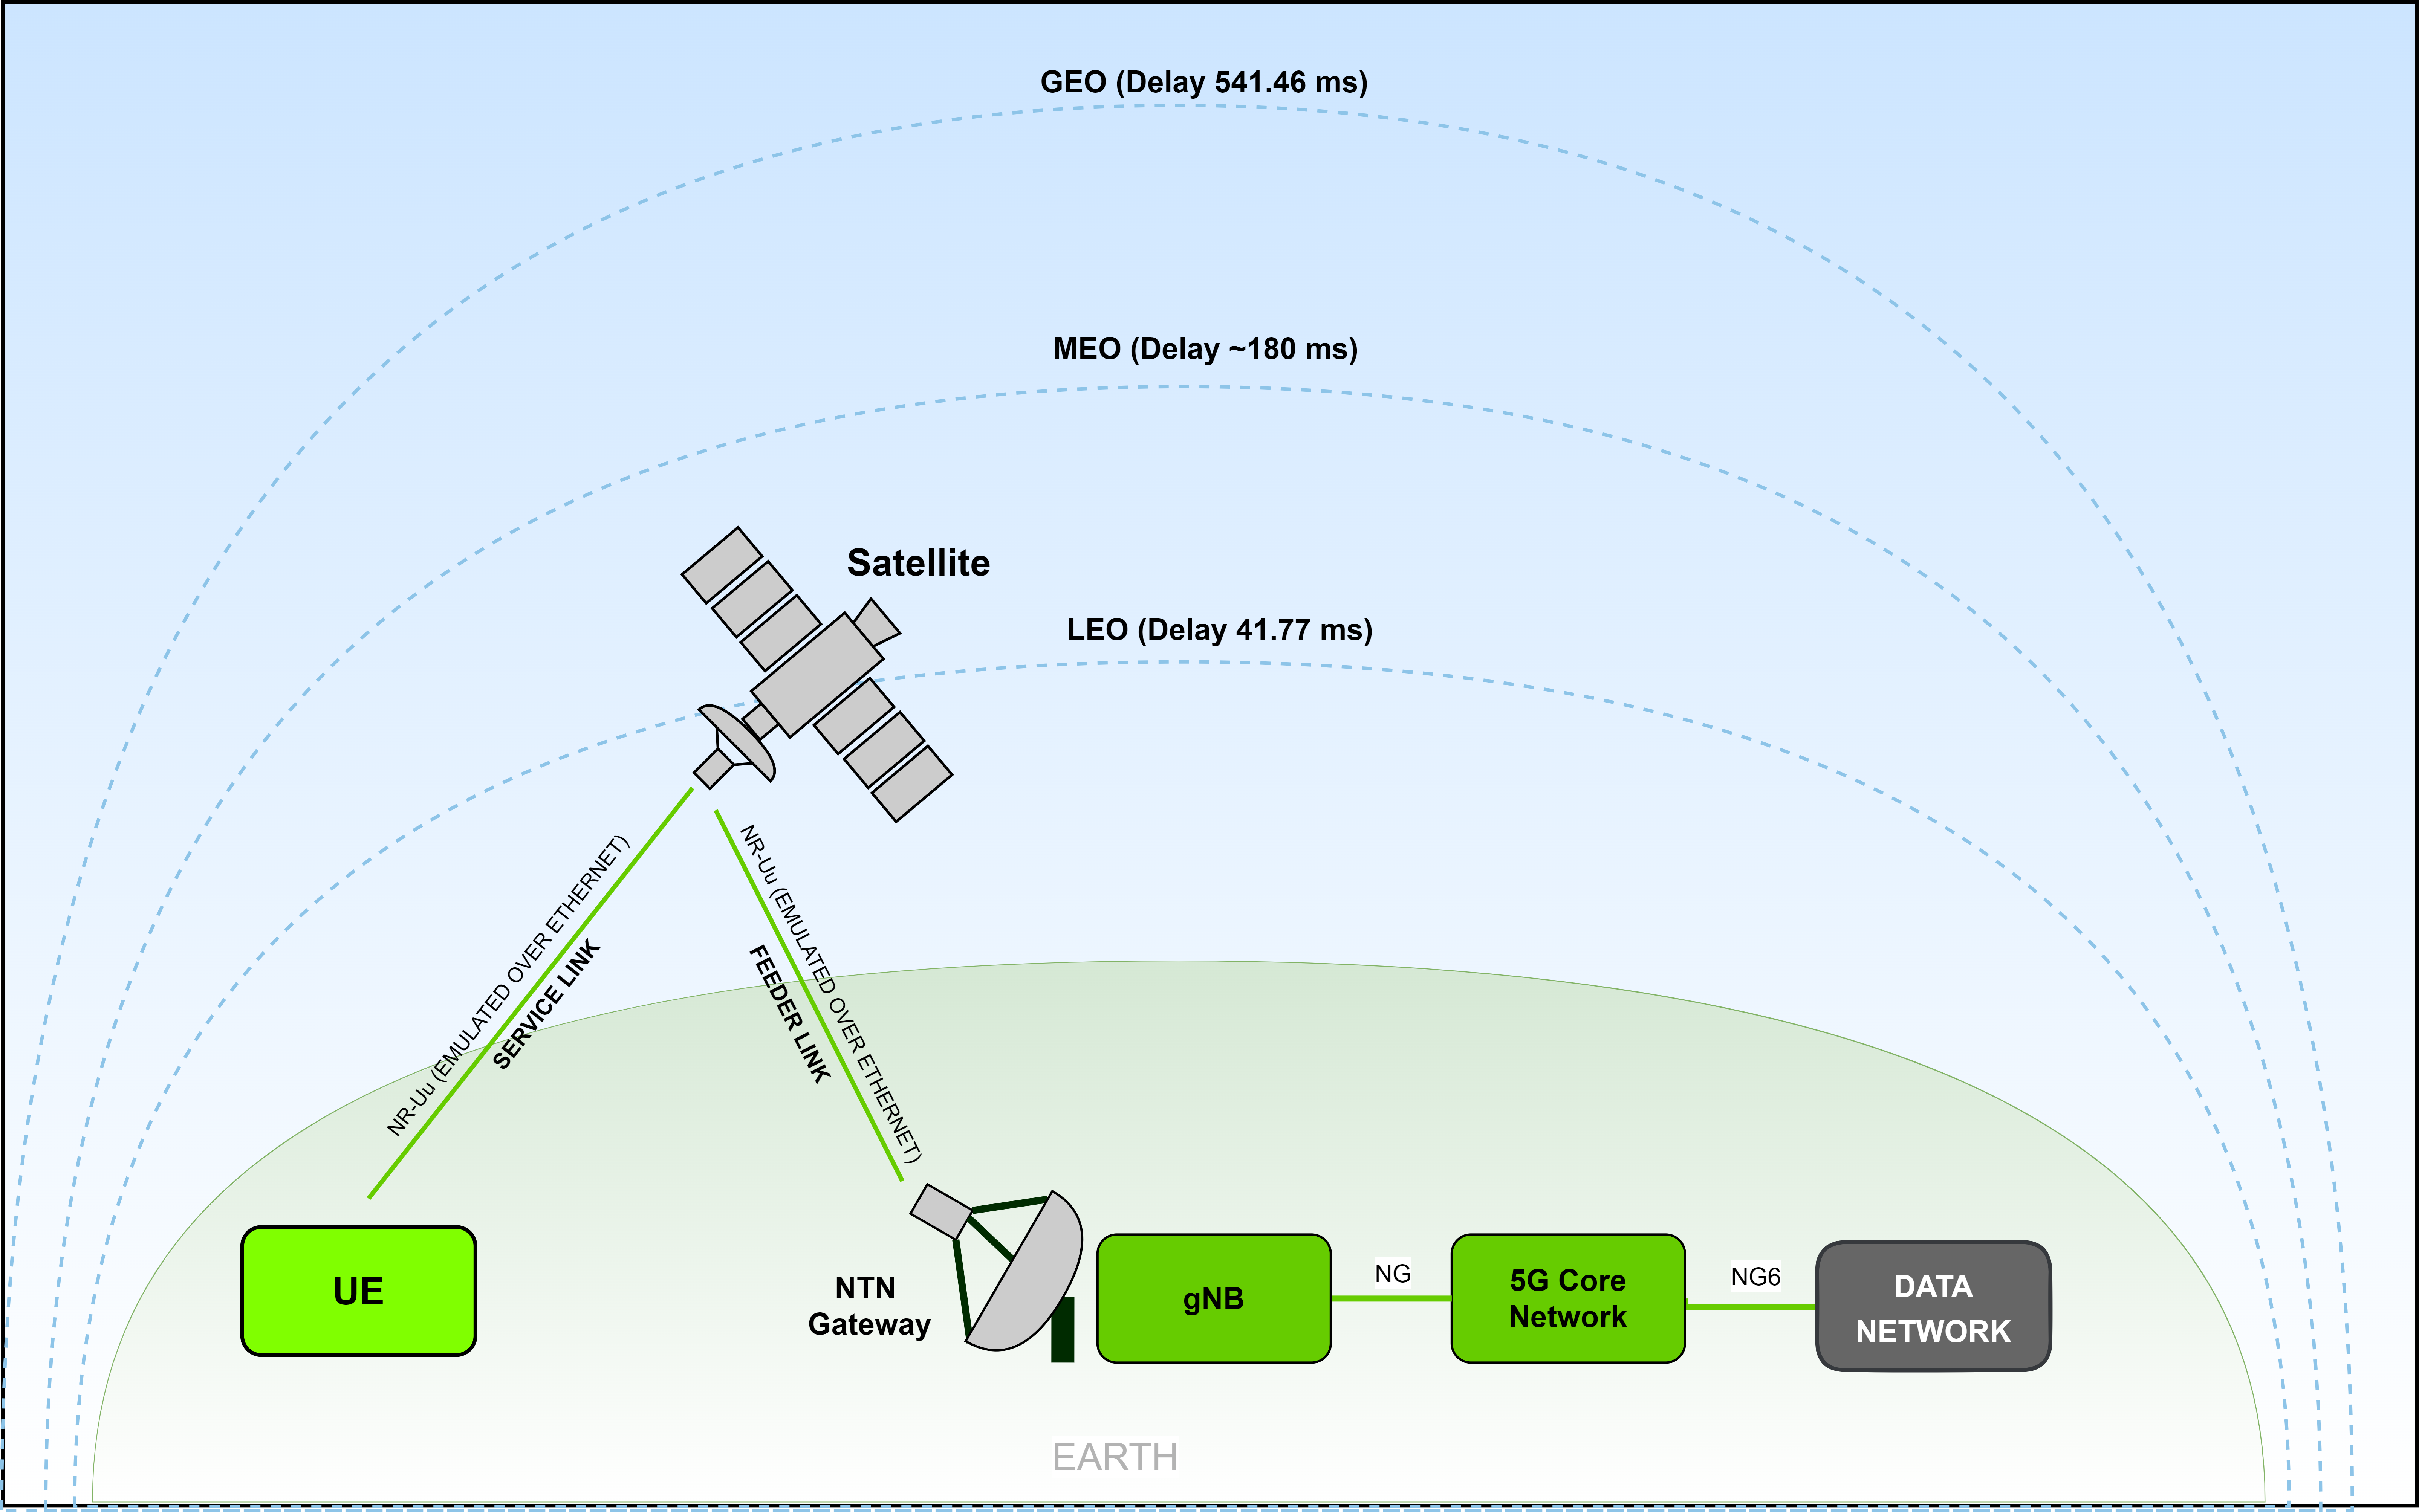
\includegraphics[width=1.05\columnwidth]{./Figures/SATCOM_figure.png}
\caption{Transparent satellite based NG-RAN architecture}
\label{SATCOM_figure}
\end{figure}

There can be various types of satellites, these are compared in Table \ref{comparison_table_between_satellites}:
\begin{table}[H]
\centering
\begin{tabular}{|c|c|c|c|}
\hline
\textbf{PARAMETER}                                                           & \textbf{GEO}     & \textbf{MEO}      & \textbf{LEO}          \\ \hline
Altitude                                                                     & 36000 km         & 7000 to 25000 km  & 300 to 1500 km        \\ \hline
\begin{tabular}[c]{@{}c@{}}Round trip delay \\ in milli-seconds\end{tabular} & High (541.46 ms) & Low ($\sim$180ms) & Very low (41.77 ms)   \\ \hline
Earth area coverage                                                          & Very large       & Large             & Low                   \\ \hline
Satellites required                                                          & 3 Satellites     & 6 Satellites      & Hundreds of Satellite \\ \hline
\end{tabular}
\caption{Comparison between GEO, LEO and MEO}
\label{comparison_table_between_satellites}
\end{table}
\subsection{Application of SATCOM based UAV}
A UAV with SATCOM capability can take on a far wider range of tasks, restricted only by its fuel capacity. For example: 
\begin{itemize}
	\item A UAV can be used by an oil business, utility, or farming company to do field inspections or deliver crucial products to remote locations hundreds of miles away from the operator. 
	\item From the next state, a defence or national security team can deliver a key part to reservists during a training drill or monitor the border with video or infrared cameras.
	\item From a remote command center, Monitoring person can get a real-time bird's eye view of a fire, accident, or medical emergency before the rescue team arrives. This will greatly help in search and rescue operations.
	\item From anywhere in the world, disaster relief groups may transport supplies to flood, hurricane, or earthquake victims and assess the situation through streaming video.
\end{itemize}

\section{Set-up for Demonstration of SATCOM}
This section gives details on the set-up used to emulate SATCOM for UAV using 5G system. The set-up consists of three Linux-x86 workstations connected over LAN. These workstations function as UE, gNB and 5G core respectively. Figure xx shows the three entity along with the software stack at each entity.

%Figure here


In a conventional 5G system, the UE and gNB  communicate over wireless interface called the Uu interface. However, in our set-up this interface is emulated using raw socket connection over LAN. Futher, the connection between the gNB and the 5G core is also over the raw socket. Since, we are using raw socket to transfer the control and data packets between the entities, the PHY layer which perform functions such as amplication, coding, modulation, etc is not needed. Hence, the PHY layer is not implemented in this set-up.

Software stack for all other layers (MAC, RLC, PDCP, SDAP, RRC, NAS) are present at both UE and gNB. An open source software called Free5GC is used as 5G core in our set-up, whose main task includes: Radio resource allocation, control and initial set-up of UE, authenticates subscribers and devices, applies personalized policies, manages the mobility of the devices, etc.

\section{Video Streaming using SATCOM} 
\subsection{FREE-5GC}
Make sure the FREE-5GC is running. Follow the document named Doc to set up and run FREE-5GC.
\subsection{gNB}
\textbf{NOTE :} For Pre-requisites and detailed installation steps , Please refer to the file \textbf{\"UE\_ gNB\_ setup\_ user\_ guide.docx\"}.
After pre-requisite installations (JSON, ROHC, Nettle, Libexplain, DPDK, ASN1, SCTP, AESN1 and IPSEC), Follow the below steps in gNB workstation terminal:

\subsubsection{Exporting environment variables:}

\begin{lstlisting}
export RTE_SDK=<path to DPDK folder installed>
export RTE_TARGET=x86_64-native-linuxapp-gcc
\end{lstlisting}

\subsubsection{Loading Huge pages:}
\begin{lstlisting}
sudo su
echo 4096 > /sys/kernel/mm/hugepages/hugepages-2048kB/nr_hugepages
exit
\end{lstlisting}

\subsubsection{Compiling and running the gNB App:}
\begin{lstlisting}
cd ~/Documents/simran_wsp/bs_working/review-bs/5gnrps/src/gnbapp/test
make clean
make static -j10
sudo ./gnbapp enp1s0 -- -diersg
\end{lstlisting}

\subsection{UE}
\textbf{NOTE :} For Pre-requisites and detailed installation steps , Please refer to the file \textbf{"UE\_gNB\_setup\_user\_ guide.docx"}.
After pre-requisite installations (JSON, ROHC, Nettle, Libexplain, DPDK, ASN1, SCTP, AESN1 and IPSEC), Follow the below steps in gNB workstation terminal:

\subsubsection{Exporting environment variables:}
\begin{lstlisting}
export RTE_SDK=/home/greyteal/Documents/6G_Project/dpdk-stable-20.02.1
export RTE_TARGET=x86_64-native-linuxapp-gcc
\end{lstlisting}

\subsubsection{Loading Huge pages:}
\begin{lstlisting}
sudo su
echo 4096 > /sys/kernel/mm/hugepages/hugepages-2048kB/nr_hugepages
exit
\end{lstlisting}

\subsubsection{Compiling and running the UE App:}
\begin{lstlisting}
cd /home/greyteal/Documents/simran_wsp/UE/5gnrps/src/ueapp/test
make clean
make CPUSOC=1 JSON=1 -j10
sudo ./ueapp enp1s0 0 -- -dierns
\end{lstlisting}

\subsubsection{Note the PDU session IP address and open a seperate terminal to run the following commands:}
\begin{lstlisting}
sudo ifconfig tun00 10.60.0.1 up
sudo ip route add 192.168.134.224 dev tun00
\end{lstlisting}

Check the PDU session using ping (5 packets):
\begin{lstlisting}
ping -I tun00 192.168.134.224 -c 5
\end{lstlisting}

\subsection{Addition of delays over Ethernet to emulate Satellite link}
Use the following commands to add delay of 542 ms at the Ethernet interface of gNB:
\begin{lstlisting}
sudo tc qdisc add dev enp2s0 root netem delay 542ms
\end{lstlisting}


Note: Other commands to show and delete the added interface delay are as follow:
\begin{lstlisting}
tc qdisc show
sudo tc qdisc del dev enp2s0 root netem
\end{lstlisting}

\subsection{Streaming video from 5GC to UE via gNB}
\subsubsection{Creating video stream at source}
To create a video stream (using file videoplayback.mp4) from 5GC to UE via gNB, run the following command in terminal of 5GC workstation. This will use UDP to stream video to a given destination IP address and port number.
\begin{lstlisting}
cd ~/Documents #go to video path
vlc videoplayback.mp4 --sout=udp://10.60.0.1:1234
\end{lstlisting}
\subsubsection{Viewing video stream at the destination}
The video packets streamed by source travel through the software stack as shown in Figure xx.
To view the stream at destination, run the following command in terminal. This will read the video packets received at the tun00 interface from the SDAP layer of software stack.
\begin{lstlisting}
vlc udp//@:1234 --miface=10.60.0.1:1234
\end{lstlisting}

